\documentclass[12pt]{article} 
\usepackage[utf8]{inputenc}
\usepackage[T1]{fontenc}
\usepackage[french]{babel}
\usepackage{geometry} 
\geometry{a4paper} 

\usepackage{graphicx} 

\usepackage{float} 
\usepackage{wrapfig}

\linespread{1.2}

\setlength\parindent{2.5pt}

\graphicspath{{Pictures/}} 

\begin{document}
\begin{titlepage}
\newcommand{\HRule}{\rule{\linewidth}{0.5mm}}
\center 

\textsc{\LARGE Universtité de Lorraine}\\[1.5cm] 
\textsc{\Large Projet Tutoré}\\[0.5cm]
\textsc{\large ASRALL}\\[0.5cm]

\HRule \\[0.4cm]
{ \huge \bfseries Systèmes de Fichiers Distribués}\\[0.4cm] 
\HRule \\[1.5cm]

\begin{minipage}{0.4\textwidth}
\begin{flushleft} \large
\emph{Author:}\\
Ricardo \textsc{RODRÍGUEZ}\\
Julien \textsc{SCHNEIDER}\\
Jean \textsc{LUTZ}\\
Yannick \textsc{LAPREVOTTE}\\
\end{flushleft}
\end{minipage}
~
\begin{minipage}{0.4\textwidth}
\begin{flushright} \large
\emph{Supervisor:} \\
 Stephane \textsc{CASSET} 
\end{flushright}
\end{minipage}\\[4cm]

{\large \today}\\[3cm] 

\vfill 
\end{titlepage}

\tableofcontents 

\newpage 

\section{Introduction} 
\section{CEPH}
\subsection{Présentation}
	Ceph est un système de fichier open-source, développé à partir d'un algorithme de nouvelle
génération appelé CRUSH \footnote{Ceph est propulsé par CRUSH (Controlled Replication Under Scalable Hashing), un algorithme de hash dérivé de la famille des algorithmes RUSH.}. Il est évolutif (\textit{scalable}) et est capable de fonctionner sur un parc de machines très diverses, on appelle ces parc de machines un cluster Ceph. Son fonctionnement repose sur 3 types de serveurs :

\begin{description}
\item[les OSDs \textit{(Object Storage Deamon "OSD")}:] sont les serveurs de stockage. Les données seront donc enregistrées sur ces nœuds. Il est préférable d'avoir une bonne quantité d'espace disque, car les OSDs journalisent les opérations d'écritures en donnée ce qui prend de la place de stockage. Il faut au minimum 2 OSDs pour que le cluster Ceph soit opérationnel.
 \item[Les Monitors \textit{(Ceph Monitor)}:] ceux-ci sont en place pour surveiller que tout fonctionne correctement. Lorsque l'on dispose d'un réseau conséquent en nœuds, il est important de savoir très rapidement quand il y a un soucis quelque part. Il est mieux d'avoir plusieurs Monitors dans le cluster Ceph pour permettre de repérer plus rapidement les erreurs et avoir un bon niveau de tolérance aux pannes. Les monitors sont des daemons relativement léger et ne nécessite pas une grande quantité de mémoire ou d'espace disque.
\item[Les MDS \textit{(MetaData Server)}:] C'est le troisième type de serveur. Celui-ci détient toutes les informations permettant de trouver les données demandées et leurs attributs. Ces informations sont très souvent consultées, elle sont dont stockées en mémoires pour en amélioré l'accès. Il faut donc une grande quantité de RAM sur les ordinateur qui hébergent les MDS.
\end{description}

Attention il n'est pas encore recommandé de l'utiliser en production : celui-ci est encore en phase de développement.
\newpage
	\subsection{Architecture du cluster}
	Nous avons choisit d'installer une configuration nous permettant de tester les performances de Ceph. Comme dit précédemment, Ceph a besoin de 3 types de nœuds différents. Nous avons choisit d'utiliser 6 machines pour 9 noeuds, ces machines seront utilisé sous Debian :
\\\\-La première machine sera l'Admin node, elle contiendra aussi le premier monitor et le premier OSD :
\begin{verbatim}
nom machine : golem
ip : 192.168.1.51
\end{verbatim}

- La deuxième machine contiendra le deuxième Monitor et le second OSD :
\begin{verbatim}
nom machine : rondoudou 
ip :  192.168.1.29
\end{verbatim}

- La troisième machine contiendra le troisième Monitor et le troisième OSD :
\begin{verbatim}
nom machine : behemot
ip :    192.168.1.56
\end{verbatim}

- La quatrième machine contiendra le premier MDS :
\begin{verbatim}
nom machine : carapuce 
ip : 192.168.1.43
\end{verbatim}

- La cinquième machine contiendra le deuxième MDS :
\begin{verbatim}
nom machine : smogogo
ip : 192.168.1.2
\end{verbatim}

- La sixième machine contiendra le troisième MDS :
\begin{verbatim}
nom machine : porygon
ip : 192.168.1.48
\end{verbatim}

Nous avons également dû installer les clients qui utilise ce cluster nous les avons installé sur nos machines personnelles.

	\subsection{Installation}
	
	Ceph a été créer pour fonctionner sur du matériel de base, pas besoin d'avoir de grosse configuration ou de matériel spécifique pour faire tourner ceph, ce qui rend la construction et le maintien d'un cluster de données de l'ordre du pétaoctets \footnote{Un pétaoctet contient \begin{math}10^{15}\end{math} octets} facilement et économiquement réalisable.
	Pour l'installation de Ceph, il faut d'abord configurer le matériel que nous allons utiliser.

 \subsubsection{Recommandation Matériel }	
	
	CPU :
	MDS : Les serveurs de métadonnée \footnote{c'est une donnée servant à définir ou décrire une autre donnée quel que soit son support} redistribue dynamiquement leur metadonnée, ce qui utilise une grande quantité de puissance processeur \textit{CPU} \footnote{est le composant de l'ordinateur qui exécute les instructions machine des programmes informatiques.}. Les MDS doivent avoir un assez bon processeur (quad-core ou mieux).
	Osd : Les serveur de donnée ceph font tourner le service RADOS, calculent le placement des datas avec CRUSH, repliquent les données, et maintiennent des copies de la carte \footnote{Une série de cartes comportant la carte de moniteur,la carte des OSDs,la carte PG, la carte des MDS et la carte CRUSH} (\textit{map}) du cluster. Les serveur de donnée ont un besoin raisonnables de puissance CPU.
	Monitor : les monitor n'ont pas besoin de puissance CPU, ils ne font que maintenir une copie de la carte du cluster pour repérer les erreurs dans le cluster.
	
	RAM :
	La ram est surtout utilisé par les serveurs de métadonnée et les monitors, car ils doivent être capable de parcourir leur données rapidement, ils doivent donc avoir une bonne quantité de RAM. Il est recommandé d'avoir 1 GB de RAM par daemon \footnote{désigne un type de programme informatique, un processus ou un ensemble de processus qui s'exécute en arrière-plan plutôt que sous le contrôle direct d'un utilisateur.}.
	Les Osds n'utilisent pas beaucoup de RAM pour leurs fonctionnements normal, mais ils en utilisent plus si l'on lance une récupération de donnée.
	
	\subsection{Erreurs rencontrées lors de l'installation de Ceph}
	\subsubsection{Erreur lors de l'installation du premier MDS}
	Pendant notre 1ère installation de Ceph, nous avions réussit à installer :
	\\ 1 Monitor sur golem et 2 OSDs sur golem et rondoudou, mais lorsque nous avons tenté d'installer le 1er MDS avec la commande :
	\begin{verbatim}
	ceph@golem:~/cluster$ceph-deploy mds create carapuce
	\end{verbatim}
	
	Il y a eu des erreurs :
	\begin{verbatim}
	[carapuce][WARNIN] No data was received after 300 seconds, disconnecting...
Traceback (most recent call last):
  File "/usr/bin/ceph-deploy", line 21, in <module>
    sys.exit(main())
 File "/usr/lib/python2.7/dist-packages/ceph_deploy/util/decorators.py",
  line 62, in newfunc
    return f(*a, **kw)
 File "/usr/lib/python2.7/dist-packages/ceph_deploy/cli.py", line 138,
  in main
 return args.func(args)
File "/usr/lib/python2.7/dist-packages/ceph_deploy/mds.py", line 169,
 in mds
    mds_create(args)
 File "/usr/lib/python2.7/dist-packages/ceph_deploy/mds.py", line 157,
  in mds_create
    create_mds(distro.conn, name, args.cluster, distro.init)
 File "/usr/lib/python2.7/dist-packages/ceph_deploy/mds.py", line 55, 
 in create_mds
    os.path.join(keypath),
  TypeError: 'NoneType' object is not iterable 
	\end{verbatim}

Après cette erreur le cluster que nous avions installé n’était plus utilisable , la commande :
\begin{verbatim}
ceph@golem:~/cluster$ceph status
\end{verbatim}
nous a renvoyé :
\begin{verbatim}
10/02/2014 : erreur lors de la commande ceph status et ceph health
 pour vérifier le fonctionnement de ceph,les commandes renvoient :

    root@golem:~# ceph status

    2014-02-10 15:58:38.386216 7fdab0128700  0 -- :/1030939 >>
     192.168.1.51:6789/0 pipe(0x185e3c0 sd=3 :0 s=1 pgs=0 cs=0 l=1 
     c=0x185e620).fault

    2014-02-10 15:58:41.381650 7fdaa8d83700  0 -- :/1030939 >>
     192.168.1.51:6789/0 pipe(0x185d510 sd=3 :0 s=1 pgs=0 cs=0 l=1 
     c=0x185d770).fault

    2014-02-10 15:58:44.381919 7fdab0128700  0 -- :/1030939 >>
     192.168.1.51:6789/0 pipe(0x185b000 sd=3 :0 s=1 pgs=0 cs=0 l=1 
     c=0x185b260).fault

    ^CError connecting to cluster: InterruptedOrTimeoutError
\end{verbatim}

Nous avons supprimer le cluster ceph avec purge autoremove, nous avons également supprimer le cluster de l'Admin Node et les fichier de conf et nous avons lancé une réinstallation complète de ceph. Pour cette réinstallation, nous avons suivi le tutoriel du site officiel pour recommencer.
	\subsubsection{Problème de cluster}
	Problème de cluster nous avions 3 cluster de ceph installé sur golem :
	
 $ Un\ dans\ /home/root/cluster\ fsid\ =\ 490b1d93-f413-430b-b5d7-d632b7556f35$
	 
 $ Un\ dans\ /home/ceph\ fsid\ =\ 0346f25b-53f7-43ce-9018-8e37181f844d$
 
	 $ Un\ dans\ /home/ceph/cluster\ fsid\ =\ d4a63950-a12f-4e4d-983b-57583bf09bac$
	 
	 Mais lors de nos manipulations sur notre 1ére installation, nous avons lancé des commandes ceph-deploy en-dehors de notre répertoire cluster, ce qui a créer de nouveau fichier de configuration et un autre cluster instable avec un nom par défaut. Mais nous n'avions pas changer le nom par défaut de notre cluster et donc plusieurs cluster du même nom ont été créer, et les cluster en-dehors du répertoire cluster était instable, ce qui a posé problème lors du démarrage du service ceph.	

On a alors purge toute l'installation de ceph avec :
\begin{verbatim}
ceph-deploy purgedata golem rondoudou carapuce behemot porygon smogogo
ceph-deploy forgetkeys
ceph-deploy purge golem rondoudou carapuce behemot porygon smogogo
\end{verbatim}

Pour avoir un seul cluster il faut lancer toutes les commandes d'installation de ceph dans un seul dossier : /home/ceph/cluster

on a ajouter dans le .bashrc de ceph des alias :
\\ alias ceph-deploy='cd /home/ceph/cluster; ceph-deploy' 
\\ alias ceph='cd /home/ceph/cluster; ceph' 

	\subsubsection{Problème de l'horloge système des machines}
Vers la fin de notre projet nos machines on eu un décalage d'horloge (\textit{clock skew}) de quelque seconde, ce qui empêché ceph de fonctionner normalement, Ceph est comme un file system \footnote{c'est une façon de stocker les informations et de les organiser dans des fichiers} mais sur plusieurs machines si ces machines n'ont pas une horloge synchronisé, la copie de fichier peut causer des problèmes. Pour palier ce problème nous avons dû reconfigure ntp :
\begin{description}
\item[Serveur NTP \textit{(Network Time Protocol "NTP")}:] 
On a fait un serveur ntp sur golem en modifiant le fichier /etc/ntp.conf en enlevant les serveur de temps extérieur et en rajoutant golem comme serveur :

\begin{verbatim}
  Fichier /etc/ntp.conf
server 127.127.1.0 # adresse localhost utilisé par ntp
server 192.168.1.51 # adresse de golem pour le nommé comme serveur ntp
fudge 127.127.1.0 stratum 4 # ajouter l'horloge système comme source 
de temps par le paramètre fudge et pour le mettre en stratum 4

restrict 192.168.1.0 mask 255.255.255.0  nomodify # pour restricter
l’accès au serveur et ne permettre qu'aux machine sur le réseau
de se synchroniser sur le serveur ntp

broadcast 192.168.1.255 # l'adresse de broadcast 
\end{verbatim}

Le serveur ntp est fonctionnel, il permet de diffuser son horloge sur les clients.
\item [Client NTP :]
L'installation du client ntp se fait avec apt:
\begin{verbatim}
apt-get install ntpdate
\end{verbatim}

Nous avons ensuite lancé une mise à jour de l'horloge des client à partir du serveur ntp sur golem avec l'aide de :
\begin{verbatim}
ntpdate 192.168.1.51
\end{verbatim}
 (nous avons lancé plusieurs fois cette commande pour accélérer la synchronisation de toute les horloges)
et ensuite nous avons modifié le fichier /etc/ntp.conf pour rajouter le serveur ntp sur les clients :
\begin{verbatim}
  Fichier /etc/ntp.conf
server 192.168.1.51 
\end{verbatim}

Nos machines sont donc toutes synchronisée à partir de golem et nous n'avons plus de problème décalage d'horloge sur Ceph.
\end{description}

	\subsection{Test de disponibilités}
	Ceph permet de facilement ajouter/supprimer de nouveaux nœud dans le cluster : comme des monitors, des osds ou des mds.

	\subsubsection{Test de surpression d'un MDS}
	Vérification du sytéme sur ceph avec le mds planté :
\begin{verbatim}
ceph@golem:~/cluster-cheese$ceph health 
    HEALTH_WARN mds carapuce is laggy  
    ceph@golem:~$ceph status     
    cluster dde8d8a9-e880-4c81-8bc6-8ede2adbe71
     health HEALTH_WARN mds carapuce is laggy 
     monmap e2: 3 mons at {behemot=192.168.1.56:6789/0,golem=
     192.168.1.51:6789/0,rondoudou=192.168.1.29:67891}, election 
     epoch 30,quorum 0,1,2 behemot,golem,rondoudou 
     mdsmap e9: 2/2/2 up {0=smogogo=up:active,1=porygon=up:active}, 
     1 down:standby(laggy or crashed)
     osdmap e44: 3 osds: 3 up, 3 in 
      pgmap v188: 192 pgs, 3 pools, 17276 bytes data, 37 objects 
            15470 MB used, 15004 MB / 30475 MB avail 
                 192 active+clean 
\end{verbatim}
	Si le mds est enlevé du cluster, il suffit de le reconnecter au réseau et de relancer le service ceph pour qu'il se réactive.
(carapuce  a planter,  on l'as relancer mais la carte réseau ne c'est pas relancer, on la lancer avec ifup eth1 et le mds remarche)

quand le mds à redémarré j'ai refait un ceph status sur golem :
\begin{verbatim}
    ceph@golem:~/cluster-cheese$ceph status     
    cluster dde8d8a9-e880-4c81-8bc6-8ede2adbe71
      health HEALTH_OK  
     monmap e2: 3 mons at {behemot=192.168.1.56:6789/0,golem=
     192.168.1.51:6789/0,rondoudou=192.168.1.29:67891}, election 
     epoch 30,quorum 0,1,2 behemot,golem,rondoudou 
     mdsmap e9: 2/2/2 up {0=smogogo=up:active,1=porygon=up:active},
      1 up:standby
      osdmap e44: 3 osds: 3 up, 3 in 
      pgmap v188: 192 pgs, 3 pools, 17276 bytes data, 37 objects 
            15470 MB used, 15004 MB / 30475 MB avail 
                 192 active+clean 
\end{verbatim}

Le MDS est de nouveau utilisable, mais il reste en standby car le mds qui l'as remplacé fonctionne bien et contient les métadonnées nécessaire pour permettre de surveiller Ceph.

	\subsubsection{Test de suppression d'un OSD}
	Nous avons enlevé 1 OSD de notre cluster, nous vérifions l'état du cluster pour voir s'il fonctionne encore :
	
	\begin{verbatim}
	ceph@golem:~/cluster-cheese$ceph status     
    cluster dde8d8a9-e880-4c81-8bc6-8ede2adbe71
       health HEALTH_WARN 192 pgs degraded; 192 pgs stale; 192 pgs stuck
     stale; 192 pgs stuck unclean; 1/1 in osds are down  
     monmap e2: 3 mons at {behemot=192.168.1.56:6789/0,golem=
     192.168.1.51:6789/0,rondoudou=192.168.1.29:67891}, election 
     epoch 30,quorum 0,1,2 behemot,golem,rondoudou 
     mdsmap e9: 2/2/2 up {0=smogogo=up:active,1=porygon=up:active},
      1 up:standby
      osdmap e44: 3 osds: 2 up, 2 in 
      pgmap v188: 192 pgs, 3 pools, 12476 bytes data, 37 objects 
            10235 MB used, 10002 MB / 20350 MB avail 
                 192 stale+clean+degraded
\end{verbatim}	 

on a donc réactivé l'osd manquant :
\begin{verbatim}
ceph-deploy osd activate rondoudou:sda3
\end{verbatim}
le système ceph est de nouveau "fonctionnel" après ces manipulations. 
\begin{verbatim}
ceph@golem:~/cluster-cheese$ceph status     
    cluster dde8d8a9-e880-4c81-8bc6-8ede2adbe71
      health HEALTH_OK  
     monmap e2: 3 mons at {behemot=192.168.1.56:6789/0,golem=
     192.168.1.51:6789/0,rondoudou=192.168.1.29:67891}, election 
     epoch 30,quorum 0,1,2 behemot,golem,rondoudou 
     mdsmap e9: 2/2/2 up {0=smogogo=up:active,1=porygon=up:active},
      1 up:standby
      osdmap e44: 3 osds: 3 up, 3 in 
      pgmap v188: 192 pgs, 3 pools, 17276 bytes data, 37 objects 
            15470 MB used, 15004 MB / 30475 MB avail 
                 192 active+clean 
\end{verbatim}
    
	\subsection{Test de performances}
	
	
  
\section{Lustre}

\begin{figure}[H] 
\center{
\includegraphics[width=0.5\linewidth]{placeholder}}
\caption{Lustre F.S.}
\label{fig:speciation}
\end{figure}

\subsection{Introduction}
Lustre est un système de fichiers distribué libre(sous licence GPL v2), utilisé pour de très grandes grappes de serveurs. Son nom vient de la combinaison de deux mots, «Linux» et «cluster». Le projet a commencé comme un projet de recherche en 1999 par Peter Braam, en 2007 Sun Microsystems a continué son développement, en 2010 avec l'acquisition de Sun, a commencé à manternir et sortir nouvelles versions de Lustre, en décembre du 2010 Oracle a arrêté le développement du système de fichiers version 2.x, plusieurs nouvelles organisations surgirent à fournir un soutien et de développement dans un modèle de développement communautaire ouvert, comprenant \textit{Whamcloud}, \textit{Open Scalable File Systes, Inc. (OpenSFS)}, \textit{EUROPEAN Open FileSystems (EOFS)} et autres. En 2012 WhamCloud a été rachetée par Intel.\\


Lustre a la possibilité de accueillir des dizaines de milliers de systèmes client et une grande quantité de données, pétaoctets\footnote{Un pétaoctet contient \begin{math}10^{15}\end{math} octets} de stockage et des centaines de gigaoctets(Go) de débit Entrée/Sortie. 

\subsubsection{Les composants de Lustre}
\begin{description}
\item[Serveur de Métadonnées \textit{(Metadata Server «MDS»)}:]
Le serveur MDS rend les métadonnées, stockées dans un ou plusieurs MDT, disponibles pour des clients Lustre. Chaque MDS gère les noms et répertoires dans le systèmes de fichiers Lustre.
\item[Cible de Métadonnées \textit{(Metadata Target «MDT»)}:] Le MDT stocke les métadonnées(tels que les noms de fichiers, les répertoires et la structure des fichiers) sur un MDS. Chaque système de fichiers possède un MDT. Une MDT sur une cible de stockage partagé peut être disponible pour de nombreux MDS, bien que l'on devrait utiliser effectivement. Si une MDS actif échoue, un MDS passif peut servir le MDT et le rendre disponible aux clients. Ceci est appelé \textit{MDS failover}.
\item[Serveur de Stockage d'Objets \textit{(Object Storage Server «OSS»)}:]
L'OSS fournit un servicce d'Entrée/Sortie de fichiers et \textit{network request handling} pour un ou plusieurs OST locaux. Typiquement, un OSS sert entre 2 et 8 OST, jusqu'à 8 To\footnote{Un téraoctet contient \begin{math}10^{12}\end{math}octets.}
\item[Cible de Stockage d'Objets \textit{(Object Storage Target «OST»)}:]
L'OST stocke les données(des morceaux de fichiers de l'utilisateur) comme des objets de données sur un ou plusieurs OSS. Un seul système de fichiers Lustre peut avoir plusieurs OST, servant chacun un sous-ensamble de fichiers données. Il n'est pas nécessairement une correspondance 1:1 entre un fichier et un OST. Pour optimiser les performances, un fichiers peut être distribué sur plusieurs OST.
\item[Serveur de Gestion \textit{(Management Server «MGS»)}:]
Le MGS stocke les informations de configuration pour tous les systèmes de fichiers Lustre dans une grappe de serveurs. Chaque component Lustre contacte le MGS pour fournir information, et les Lustre clients contactent le MGS pour obtenir information.
\item[Lustre clients:]Lustre clients sont noeuds éxecutant le logiciel Lustre qui leur permet de monter le système de fichiers Lustre.

Le logiciel client de Lustre est composé d'une interfacce entre le \textit{Linux Virtual File System} et les serveurs Lustre. Chaque cible(composant de Lustre) a une contrapartie client: Client de Métadonnées (MDC), Client de Stockage d'Objets(OSC) et un Client de Gestion(MGC). Un groupe de OSC sont intégrés dans un Volume d'objets logique(\textit{Logical Object Volume «LOV»}). Travaillant en collaboration, les OSC fournissent un accès transparent au système de fichiers.

Les clients qui montent le système de fichiers Lustre, voient un seul, cohérente, espace de noms(\textit{namespace}), synchronisé toujours. Différents clients peuvent écrire aux différentes parties d'un même fichier en même temps, tandis que d'autres clients peuvent lire le fichier.
\end{description}
\subsubsection{Principales Caractéristiques de Lustre}

Les principales caractéristiques de Lustre comprennent: \\

\begin{description}

\item[Évolutivité: ]
 Lustre échelles haut ou le bas par rapport au nombre de postes clients, stockage sur disque et bande passante. Actuellement , Lustre est en cours d'exécution dans des environnements de production avec un maximum de 26 000 postes clients, avec de nombreux grappes d'entre 10,000 et 20,000 clients. Autres installations fournissent Lustre d'espace de stockage en disque agrégé et bande passsante allant jusqu'à 1000 OST fonctionnant sur plus de 450 OSS. Plusieurs systèmes de fichiers Lustre avec une capacité de 1 pétaoctet ou plus (permettant le stockage de jusqu'à 2 milliards de fichiers) ont été en usage depuis 2006.
\item[Performance: ]
 Lustre déploiements dans des environnements de production offrent actuellement la performance de jusqu'à 100 Go par seconde. Dans un environnement de test, une performance de 130 Go par seconde a étée soutenue. Lustre seul débit de poste client a été mesurée à 2 Go par seconde (max) et OSS débit de 2,5 Go par seconde (max). Lustre a été exécuté à 240 Go par seconde sur le système de fichiers d'araignée(Spider File System) à Oak Ridge National Laboratories.

\item[Conformité POSIX:]Dans un cluster, la conformité POSIX signifie que la plupart des opérations sont atomiques et les clients ne voient jamais des données périmées ou métadonnées .
\item[Haute Disponibilité:]Lustre propose des partitions de stockage partagés pour les cibles de l'OSS (OST), et une partition de stockage partagé pour la cible MDS (MDT).

\item[Sécurité:]En Lustre, il s'agit d'une option pour les connexions TCP seulement de ports privilégiés. Manipulation des membres du groupe est basée sur le serveur. POSIX listes de contrôle d'accès (ACL) sont pris en charge .
\item[Open Source:] Lustre est sous licence GNU GPL v2.
\item[]
\end{description}
\subsubsection{Lustre Network}

\textit{Lustre Network (LNET)} est une API de réseau personnalisé qui fournit l'infrastructure de communication qui gère l'Entrée/Sortie des métadonnées et fichiers de données pour les serveurs et les clients du système de fichiers Lustre.

LNET prend en charge plusieurs types de réseaux couramment utilisés, tels que les réseaux \textit{InfiniBand} et \textit{IP}, et permet la disponibilité simultanée sur plusieurs types de réseaux avec routage entre eux. Accès à la mémoire direct à distance (RDMA) est autorisée lorsqu'elle est soutenue par des réseaux sous-jacentes utilisant le pilote réseau Lustre approprié (\textit{Lustre Network Driver «LND»}). Haute disponibilité et de récupération permettent la récupération transparente avec les serveurs de basculement. 
Un LND est un pilote enfichable qui fournit un support pour un type de réseau particulier, par exemple \textit{ksocklnd} est le pilote qui implémente le\textit{TCP Scocket LND} qui prend en charge les réseaux TCP. LNDs sont chargés dans la pile de pilotes, avec une LND pour chaque type de réseau en cours d'utilisation.

\subsubsection{Réseaux Lustre}

Un réseau Lustre est composé de clients et serveurs exécutant le logiciel Lustre. Il n'a pas besoin d' être limité à un sous-réseau de LNET mais peut s'étendre sur plusieurs réseaux, le routage est possible entre les réseaux. D'une manière similaire, un réseau unique peut avoir plusieurs sous-réseaux LNET.

\subsubsection{Lustre cluster}


\begin{figure}[Cluster]
\center{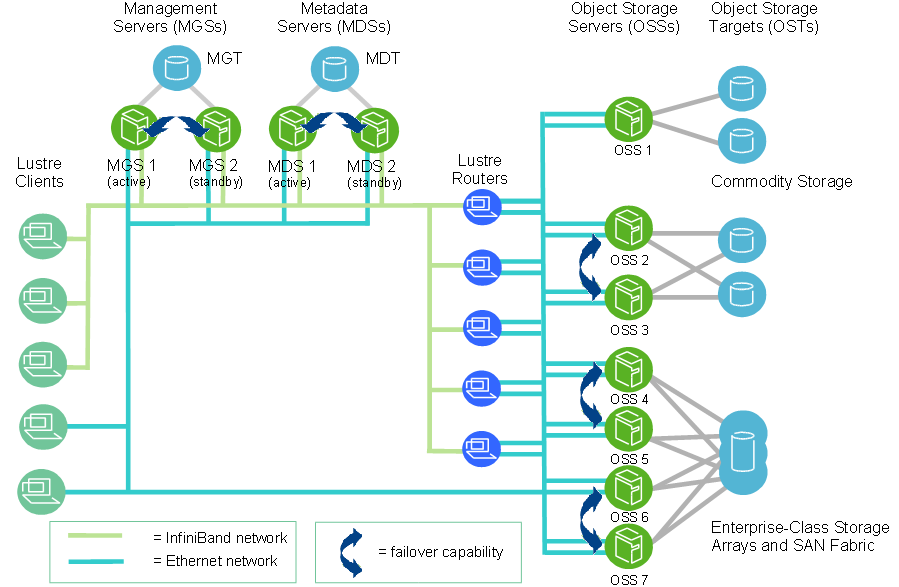
\includegraphics[width=1.0\linewidth]{scaled_cluster}}
\caption{Scaled Cluster}
\label{scaled_cluster}
\end{figure}

À grande échelle, un cluster de système de fichiers Lustre peut inclure des centaines de OSS et des milliers de clients, Figure \ref{scaled_cluster}, Plus d'un type de réseau peut être utilisé dans un cluster Lustre. Le stockage partagé entre OSS permet la fonction de basculement\textit{(failover)}.

\subsubsection{Stockage des données avec Lustre}

	Dans Lustre version 2.0, les identifiants de fichiers Lustre \textit{(File Identifier «FID») }ont été introduites pour remplacer les numéros d'inodes UNIX pour identifier des fichiers ou des objets. Un FID est un identificateur de 128 bits qui contient un numéro unique de 64 bits séquence, un 32-bit ID objet \textit{(Object Identifier «OID»)}, et un numéro de version 32 bits. Le numéro de séquence est unique parmi tous les objectifs Lustre dans un système de fichiers (OST et EMD). Ce changement a permis le soutien futur de plusieurs équipes multidisciplinaires (introduits dans Lustre version 2.3 du logiciel) et ZFS\footnote{http://fr.wikipedia.org/wiki/ZFS}(introduits dans Lustre logiciel version 2.4).\\

\begin{figure}[Donnes en Lustre]
\center{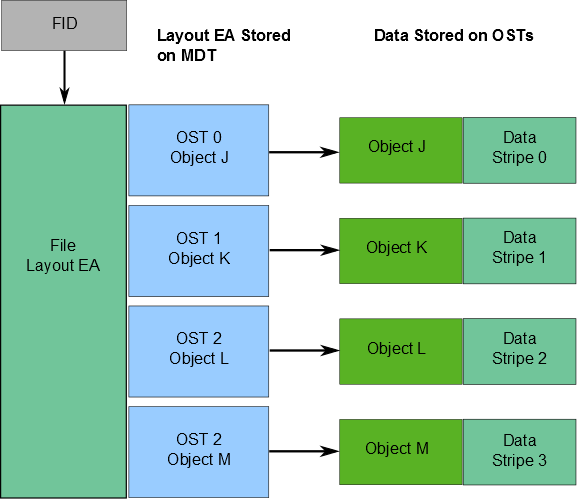
\includegraphics[width=0.5\linewidth]{dataenlustre}}
\caption{Disposition EA sur MDT pointant vers le fichier de données sur OST}
\label{dataenlustre}
\end{figure}

Informations sur l'endroit où les données de fichier se trouve sur le OST, est stockée comme un attribut étendu appelé disposition EA dans un objet MDT identifié par la FID pour le fichier(figure \ref{dataenlustre}). Si le fichier est un fichier de données (pas un répertoire ou un lien symbolique), l'objet MDT pointe de 1 à N OST objet(s) sur le(s) OST(s) qui contiennent les données de fichiers. Si le fichier MDT pointe à un objet, toutes les données de fichier sont stockées dans cet objet. Si le MDT pointe à plus d'un objet, les données du fichier sont réparties sur les objets à l'aide RAID 0, et chaque objet est stocké sur un OST différent.\\

Quand un client veut lire ou écrire dans un fichier, il récupère tout d'abord la mise en EA de l'objet MDT pour le fichier. Le client utilise ensuite ces informations pour effectuer des Entrées/Sorties sur le fichier, interagir directement avec les nœuds OSS où les objets sont stockés(Figure 4).

\begin{figure}[Client-FS]
\center{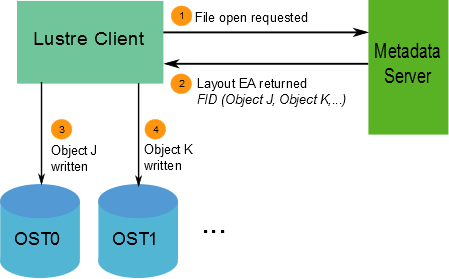
\includegraphics[width=0.6\linewidth]{file_write}}
\caption{Lustre client demandant des données}
\label{fig:identification}
\end{figure}

\newpage
\subsubsection{Lustre et l'entrelacement}

L'un des principaux facteurs menant à la haute performance des systèmes de fichiers Lustre est la capacité de répartir les données sur plusieurs OST dans un mode round-robin. Les utilisateurs peuvent éventuellement configurer pour chaque fichier le nombre de rayures, taille de bande, et OST qui sont utilisés. \\

L'entrelacement\textit{(Striping)} peut être utilisé pour améliorer les performances lorsque la bande passante globale à un fichier unique excède la bande passante d'un seul OST. La capacité de bande est également utile lorsque l'OST n'a pas assez d'espace pour contenir un fichier entier.

Le Stripping permet segments ou «morceaux» de données dans un fichier pour être stocké sur différents OST, dans le système de fichiers Lustre, une configuration RAID 0 est utilisée dans laquelle des données sont «striped» à travers un certain nombre d'objets. Le nombre d'objets dans un seul fichier est appelé \textit{stripe\_count}.

Chaque objet contient un bloc de données à partir du fichier. Lorsque le bloc de données en cours d'écriture à un objet particulier dépasse la \textit{stripe\_size}, le prochain bloc de données dans le fichier est stocké sur l'objet suivant.

Les valeurs par défaut pour \textit{stripe\_count} et \textit{stripe\_size} sont fixés pour le système de fichiers. La valeur par défaut pour \textit{stripe\_count} est une bande de fichier et la valeur par défaut pour \textit{stripe\_size} est 1Mo. L'utilisateur peut modifier ces valeurs sur une base par répertoire ou par fichier.

La taille maximale de fichier n'est pas limité par la taille d'une cible unique. Dans un système de fichiers Lustre, les fichiers peuvent être réparties sur plusieurs objets (jusqu'en 2000), et chaque objet peut être jusqu'à 16 To en taille avec ldiskfs\footnote{http://wiki.lustre.org/lid/ulfi/ulfi\_ldiskfs.html}. Cela conduit à une taille de fichier maximale de 31,25 pétaoctets. (Notez qu'un système de fichiers Lustre peut supporter des fichiers jusqu'à \begin{math}2^{64}\end{math} octets selon le stockage de sauvegarde utilisé par OST.)

\begin{figure}[Striping]
\center{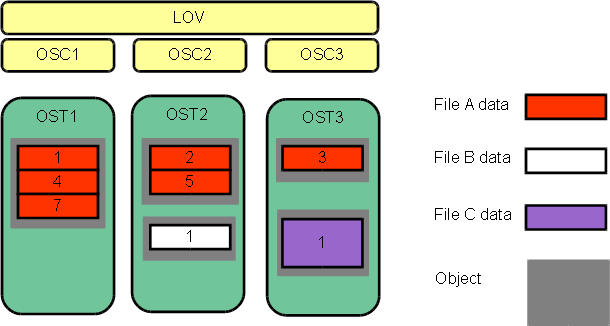
\includegraphics[width=0.6\linewidth]{file_striping}}
\caption{Striping}
\label{fig:identification}
\end{figure}


\newpage
\subsection{Installation}
\newpage
\subsubsection{Ubuntu-Lustre}
Parallèlement à la première tentative d'installation sur CentOS 6.5, en suivant la recommandation de notre tuteur, nous avons decidé de déployer les client Lustre dans une architecture virtualisée, mais en utilisant le système d'exploitation Ubuntu 13.10 cette fois.

Nous avons travaillé également avec KVM et l'outil graphique virt-manager pour créer une machine Virtuelle à laquelle nous avons attibué 7 cpus, 2 Go de mémoire vive et 20 Go de disque dur, cette machine etait destinée principalement à la compilation du noyau Linux version 3.13.6, qui donne la posibilité d'activer les frivers compatibles avec Lustre.

Le plan était compiler et installer le nouveau nouyau su cette machine et despuis les sources compiler les paquets nécesaires pour l'installation de Lustre sur chaque noeud, cloner la machine 2 fois, réduire ses resources pour les donner 2 cpus à chaqune et 1 Go de mémoire vive, deployer sur les machines clonées et la première machine les clients Lustre.

Nous avons commencé pour la compilation du noyau Linux v13.13.6, la dernière version «stable», nous sommes allés sur le site officiel\footnote{https://www.kernel.org/} pour télécharger les paquets sources.

On a obtenu le fichier «linux-3.13.6.tar.xz» dans notre machine virtuelle, pour extraire le contenu nous avons utilisé la commande:

\begin{verbatim}
	rsmrg@LUT:$tar -Jxvf linux-3.13.6.tar.xz
\end{verbatim}

Ensuite on a changé le répertoire pour nous déplacer vers celui que nous avons extrait du fichier, aussi on a installé les outils de compilation:

\begin{verbatim}
rsmrg@LUT:$cd linux-3.16.6 ; sudo apt-get install debconf-utils dpkg-dev
debhelper  build-essential kernel-package libncurses5-dev
\end{verbatim}

Nous avons copié la configuration du noyau précédant, après on a exécuté, make oldconfig pour répondre aux nouvelles questions de configurations du noyau:

\begin{verbatim}
rsmrg@LUT:$sudo cp /boot/config- 'uname -r' .config
rsmrg@LUT:$make oldconfig
\end{verbatim}

Pour activer les options Lustre on est allé au menu de configuration de noyau dans la partie «Staging drivers» (figure \ref{kernel}).

\begin{verbatim}
rsmrg@LUT:$make menuconfig
\end{verbatim}

\begin{figure}[Lustre Options]
\center{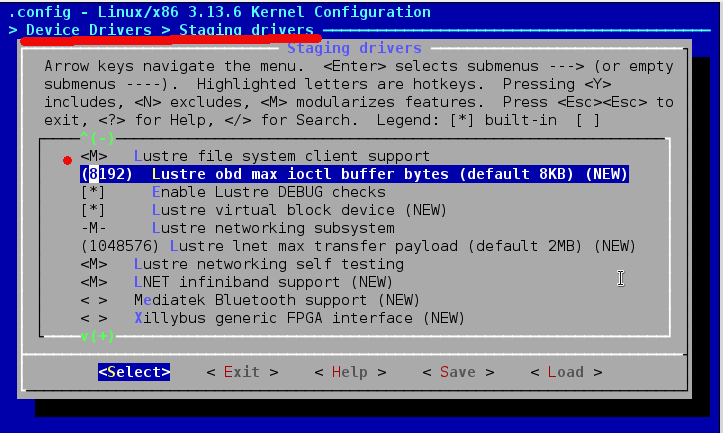
\includegraphics[width=0.8\linewidth]{kernel}}
\caption{Lustre Drivers}
\label{kernel}
\end{figure}

Après sauvegarder les manipulations réalisées, il fallait compiler le noyau en utilisant les 7 cpus et générer les paquets «.deb»:

\begin{verbatim}
rsmrg@LUT:$sudo make -j7 deb-pkg
\end{verbatim}

\begin{figure}[Compilation]
\center{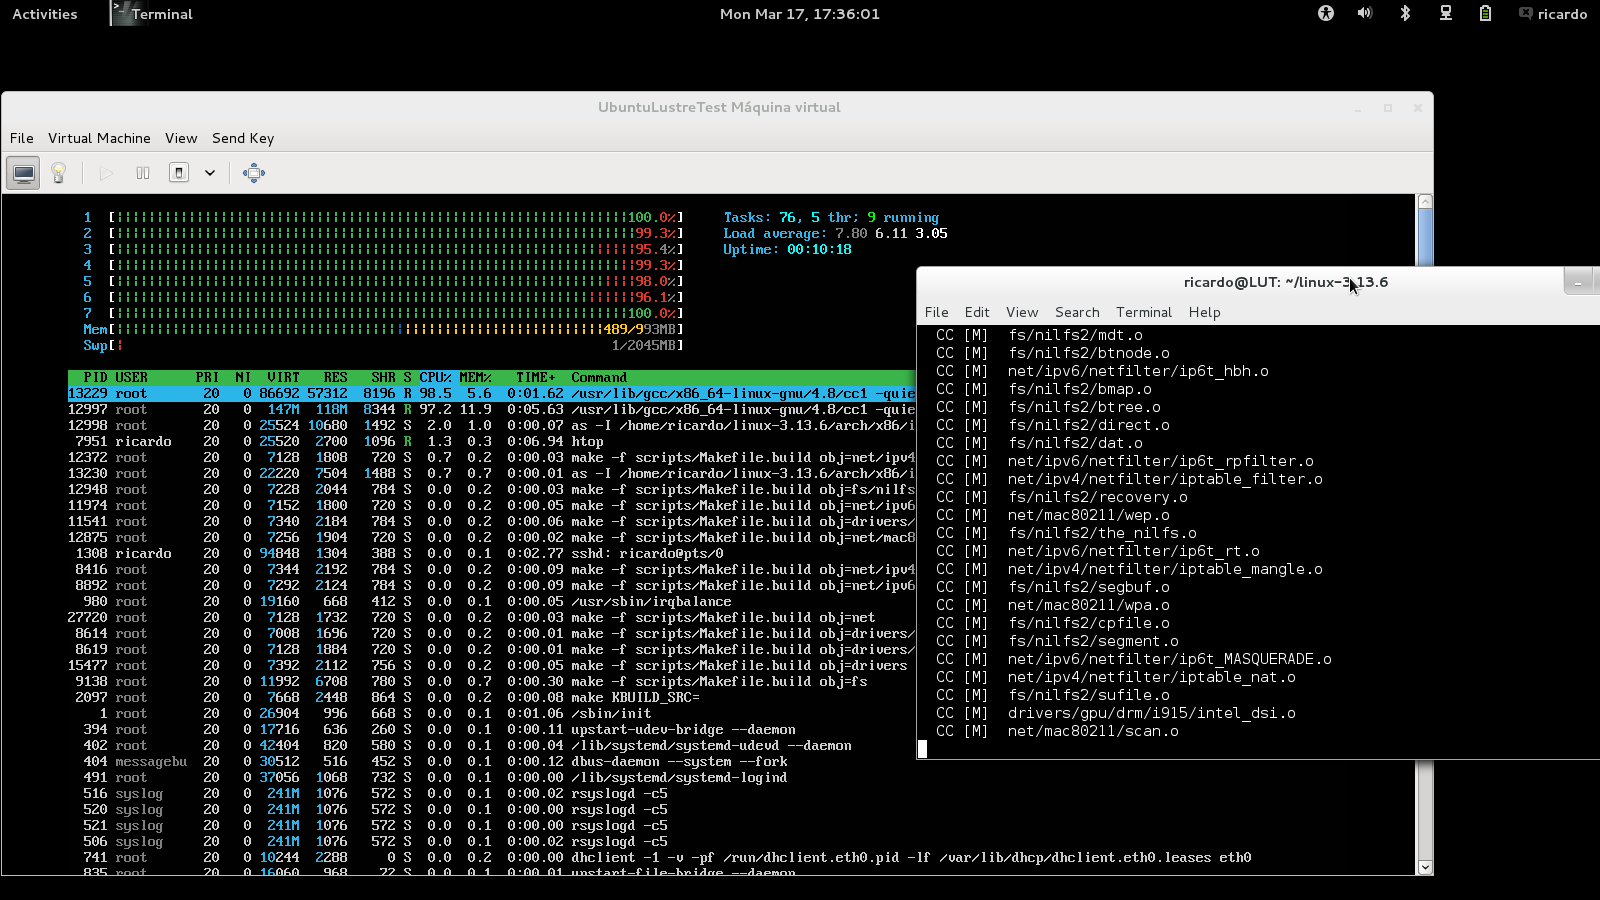
\includegraphics[width=0.8\linewidth]{compilation}}
\caption{Compilation Linux-13.13.6}
\label{kernel}
\end{figure}

Installation du nouveau kernel depuis les paquets généres:

\begin{verbatim}
rsmrg@LUT:$sudo dpkg -i ../*.deb
\end{verbatim}

Après la compilation du noyau de Linux on a essayé d'installer les paquets Lustre sur le système d'exploitation, mais sans succès, après avoir parlé avec le tuteur du projet, il a recommandé l'arrêt de travail avec Ubuntu pour  ne pas perdre plus de temps et de nous consacrer entièrement au déploimeent de Lustre avec logiciels plus anciens, mais supportés, comme c'est le cas du système d'exploitation CentOS 6.3.

\newpage
\subsection{QQLiéeàLustre}
\subsection{MásPerca}
\subsection{Lustre}
\subsection{Faru}

\section{Annexe}
 
  \subsection{How to install ceph}
	\subsubsection{Partitionnement}
	En premier, on a partitionné les machines sur lesquels un OSD sera installé, nous avons créer de nouvelle partition en xfs \footnote{est un système de fichiers 64-bit journalisé de haute performance} pour stocker les données du cluster avec le logiciel Gparted. Sur chaque machines nous avons fait une partition de environs 10 Go.
	\subsubsection{Configuration du Réseau }
	Sur chaque machine nous avons modifié le fichier /etc/hosts ajoutant l'alias et l'adresse IP \footnote{est une famille de protocoles de communication dans le domaine du réseau informatique conçus pour être utilisés par Internet.} de chaque machine ainsi elles peuvent facilement se connecter entre elles en indiquant ses alias.
	\begin{verbatim}
  Fichier /etc/hosts :
#Ceph cluster
192.168.1.51 golem
192.168.1.29 rondoudou
192.168.1.56 behemot
192.168.1.43 carapuce
192.168.1.2 smogogo
192.168.1.48 porygon
	\end{verbatim}

\textbf{ Création d'utilisateur ceph}
\\Ceph nécessite un utilisateur spécial pour la configuration et l'administration du cluster à partir de la machine d'administration, nous avons crée l'utilisateur ceph avec les droits d'administrateur du système.
\begin{verbatim}
root@golem:~/sudo useradd -d /home/ceph -m ceph
  Fichier /etc/sudoers :
ceph ALL = (root) NOPASSWD:ALL
\end{verbatim}

\textbf{Configuration ssh \footnote{est à la fois un programme informatique et un protocole de communication sécurisé.}}
\\Pour effectuer la gestion du cluster, les machines doivent se communiquer entre elles avec des tunnels ssh, avec l'utilisateur ceph il faut générer les clés publiques pour s'identifier avec les autres machines.
\begin{verbatim}
su ceph
ceph@golem:~/ssh-keygen
\end{verbatim}

Copier les clés sur tous les autres postes.
\begin{verbatim}
ceph@golem:~/ssh-copy-id ceph@nomdemachine
\end{verbatim}

Modifier le fichier ~/.ssh/config pour se connecter par les tunnels ssh avec l'utilisateur ceph par défaut.
\begin{verbatim}
  Fichier config :
Host golem
User ceph
Host rondoudou
User ceph
Host behemot
User ceph
Host carapuce
User ceph
Host smogogo
User ceph
Host porygon
User ceph
\end{verbatim}

\textbf{Synchronisation de l'heure des machines avec NTP }
\\Afin de prévenir un décalage d'horloge entre les nodes du cluster nous avons installé le serveur NTP sur golem qui nous permet de synchroniser l'horloge de toute les nodes :
\begin{verbatim}
ceph@golem: sudo apt-get install ntp
ceph@golem: sudo /etc/init.d/ntp restart
\end{verbatim}

Nous avons également installé lsb sur toute les machines, il permet de standardiser la structure interne des systèmes d'exploitation basés sur GNU/Linux :
\begin{verbatim}
ceph@golem:~$ sudo apt-get install lsb
\end{verbatim}

Sous Debian, l'installation de Ceph est simple car les développeurs mettent régulièrement les paquets à disposition mais les sources le sont autant.
La première étape consiste à rajouter les dépôts de Ceph pour apt-get.
Pour ce faire, rajoutez les deux lignes suivantes à la fin de votre
\begin{verbatim}
  Fichier ‘/etc/apt/sources-list’:
deb http://ceph.net/debian/ wheezy main
deb-src http://ceph.net/debian/ wheezy main
\end{verbatim} 
Seconde étape,  mettre a jour apt-get pour la prise en compte de ces nouveaux dépôts:
\begin{verbatim}
ceph@golem:~$sudo apt-get update
\end{verbatim}

Enfin, nous avons utilisez apt-get pour installer les paquets:
\begin{verbatim}
ceph@golem:~$ apt-get install ceph ceph-deploy
\end{verbatim}

On a ensuite créer un répertoire de travail, il est utilisé par l'Admin Node, nous avons créer ce répertoire dans le dossier courant de l'utilisateur ceph :
\begin{verbatim}
ceph@golem:~$ mkdir cluster-cheese
ceph@golem:~$ cd cluster-cheese
\end{verbatim}

A partir de maintenant toute les commandes utilisé pour créer le système de fichier distribué devrons être lancer dans ce dossier, sinon il est possible que l'utilisation d'une de ces commandes créer un deuxième cluster et des problèmes surviennent, si les 2 cluster ont le même nom.

\subsubsection{Création cluster et installation des monitors}

Nous allons commencer à installer les différents nodes de notre cluster ceph avec la commande :
\begin{verbatim}
ceph@golem:~/cluster-cheese$ceph-deploy new golem
 rondoudou behemot
\end{verbatim}

cette commande permet de déclarer les nodes du cluster.

Ensuite il y a l'installation de ceph sur ces nodes :
Pour lancer cette commande nous avons dû rajouter l'option --no-adjust-repos qui permet de passer les toutes les modifications du proxy \footnote{est un composant logiciel informatique qui joue le rôle d'intermédiaire en se plaçant entre deux autres pour faciliter ou surveiller leurs échanges.} sur le paquet et ira directement à l'installation du paquet :
\begin{verbatim}
ceph@golem:~/cluster-cheese$ceph-deploy install --no-adjust-repos
 rondoudou behemot 
\end{verbatim}

(ceph est déjà installé sur golem car c'est aussi notre Admin Node.)

Nous passons maintenant à l'installation des monitors, pour cela nous allons créer 1 monitors sur chacun des nodes présents (golem, rondoudou, behemot) avec la commande :
\begin{verbatim}
ceph@golem:~/cluster-cheese$ceph-deploy mon create-initial
\end{verbatim}

cette commande génère de nouveau fichier dans notre répertoire cluster-cheese :
\begin{verbatim}
ceph@golem:~/cluster-cheese$ls

ceph.conf ceph.log ceph.mon.keyring
\end{verbatim}

si on regarde ceph.conf :
\begin{verbatim}
  Fichier ceph.conf
[global]
fsid = 10c95f01-2dd2-4863-affa-60c4eafcd8d2
mon_ initial_members = golem, rondoudou, behemot
mon_host = 192.168.1.51, 192.168.1.29, 192.168.1.56
auth cluster required = cephx
auth service required = cephx
auth client required = cephx
osd_journal_size = 1024
\end{verbatim}

On vois que nos 3 monitors ont été ajouté dans la configuration du cluster.

\subsubsection{Installation des Osds}

Pour l'installation des OSD nous avons créé une partition de type xfs sur les machines golem, rondoudou et behemot, nous avons utilisé la commande :
\begin{verbatim}
ceph@golem:~/cluster-cheese$ceph-deploy disk list <nomdemachine>
\end{verbatim}

Qui permet de voir les partitions et leurs système de partitionnement sur les différents nodes.

Ensuite depuis golem on a formaté ces partitions avec les commandes :
\begin{verbatim}
ceph@golem:~/cluster-cheese$ceph-deploy disk zap golem:sda3
ceph@golem:~/cluster-cheese$ceph-deploy disk zap rondoudou:sda3
ceph@golem:~/cluster-cheese$ceph-deploy disk zap behemot:sda6
\end{verbatim}

Après avoir formaté les partitions nous avons préparé et activé les Osds :
\begin{verbatim}
ceph@golem:~/cluster-cheese$ceph-deploy osd prepare golem:sda3
ceph@golem:~/cluster-cheese$ceph-deploy osd activate golem:sda3
ceph@golem:~/cluster-cheese$ceph-deploy osd prepare rondoudou:sda3
ceph@golem:~/cluster-cheese$ceph-deploy osd activate rondoudou:sda3
ceph@golem:~/cluster-cheese$ceph-deploy osd prepare behemot:sda3
ceph@golem:~/cluster-cheese$ceph-deploy osd activate behemot:sda3
\end{verbatim}

(Pour certaine de ces commandes nous avons du rajouter l'option --overwrite-conf, pour modifier la configuration de ceph sur les nodes, 
ex: ceph-deploy --overwrite-conf osd prepare golem:sda3)

Après avoir installé les Osds nous pouvons déjà regardé si ceph est installé correctement avec la commande :
\begin{verbatim}
ceph@golem:~/cluster-cheese$ceph status     
    cluster dde8d8a9-e880-4c81-8bc6-8ede2adbe71
      health HEALTH_OK  
     monmap e2: 3 mons at {behemot=192.168.1.56:6789/0,golem=
     192.168.1.51:6789/0,rondoudou=192.168.1.29:67891}, election 
     epoch 30,quorum 0,1,2 behemot,golem,rondoudou 
      osdmap e44: 3 osds: 3 up, 3 in 
      pgmap v188: 192 pgs, 3 pools, 17276 bytes data, 37 objects 
            15470 MB used, 15004 MB / 30475 MB avail 
                 192 active+clean 
\end{verbatim}


\subsubsection{Installation des MDS}

Nous arrivons à la dernière partie de l'installation où nous allons installé les mds avec la commandes :
\begin{verbatim}
ceph@golem:~/cluster-cheese$ceph-deploy mds create carapuce smogogo
 porygon
\end{verbatim}

et nous voulons 2 mds d'actif, pour l'instant il y en a un d'actif de base on utilise la commande suivante :
\begin{verbatim}
ceph@golem:~/cluster-cheese$ceph mds set_max_mds 2
\end{verbatim}

Ensuite nous avons fait un ceph status pour voir si le système ceph était bien installé :
\begin{verbatim}
ceph@golem:~/cluster-cheese$ceph status     
    cluster dde8d8a9-e880-4c81-8bc6-8ede2adbe71
      health HEALTH_OK  
     monmap e2: 3 mons at {behemot=192.168.1.56:6789/0,golem=
     192.168.1.51:6789/0,rondoudou=192.168.1.29:67891}, election 
     epoch 30,quorum 0,1,2 behemot,golem,rondoudou 
     mdsmap e9: 2/2/2 up {0=smogogo=up:active,1=porygon=up:active},
      1 up:standby
      osdmap e44: 3 osds: 3 up, 3 in 
      pgmap v188: 192 pgs, 3 pools, 17276 bytes data, 37 objects 
            15470 MB used, 15004 MB / 30475 MB avail 
                 192 active+clean 
\end{verbatim} 

Nous avons un système ceph fonctionnel, qui nous permet de réaliser des test de disponibilité et de performance.
\\Avec la commande :
\begin{verbatim}
ceph@golem:~/cluster-cheese$ceph osd lspools
\end{verbatim}

Nous pouvons voir qu'il y a 3 "piscines" \footnote{Les piscines sont des partitions logiques pour stocker des objets.} sur notre cluster ceph, nous allons utilisé la pool rbd \footnote{fournit un accès à la couche Rados à travers un module noyaux} (\textit{Ceph’s RADOS Block Devices}), pour créer un file system est pouvoir stocké des données sur Ceph.

\subsubsection{Installation du client}
Pour l'installation du client, on a d'abord ajouté le client dans le réseau ceph grâce à ssh, on a créé un utilisateur ceph et on a installé ceph sur la machine-client à partir de golem (Admin Node) :
\begin{verbatim}
ceph@ronflex:~/$ceph-deploy install ceph-client
\end{verbatim}

On a ensuite copier la configuration de notre cluster de golem vers le client avec la commande : 
\begin{verbatim}
ceph@ronflex:~/$ceph-deploy admin ceph-client
\end{verbatim}

cette commande à copier le ceph.conf et le ceph.client.admin.keyring dans le dossier /etc/ceph sur le ceph-client.

Nous allons créer dans notre piscine rbd un nouveau périphérique bloc \footnote{organise les données de telle façon qu'il en résulte une amélioration de la flexibilité, des performances et de la fiabilité.} qui nous permettra de stocké des données, nous créons ici un bloc de 10Go dans la piscine rbd
\begin{verbatim}
ceph@ronflex:~/$prbd create foo --size 10096 --pool rbd
\end{verbatim}

Nous pouvons voir avec : 
\begin{verbatim}
ceph@ronflex:~/$rbd ls rbd 
ceph@ronflex:~/$rbd --image foo -p rbd info 
\end{verbatim}

que notre bloc a bien été créer.

Et maintenant nous lançons la commande :
\begin{verbatim}
ceph@ronflex:~/$rbd map foo -pool rbd
\end{verbatim}

pour ajouter à la map de rbd le nouveau bloc, on peut le voir avec la commande rbd showmapped, on a ensuite mit un système de fichier sur le bloc :
\begin{verbatim}
ceph@ronflex:~/$mkfs.ext4 -m0 /dev/rbd/rbd/foo
\end{verbatim}

et nous avons finalement monter le bloc sur le système client avec :
\begin{verbatim}
ceph@ronflex:~/$mkdir /mnt/rbd_foo
ceph@ronflex:~/$mount /dev/rbd/rbd/foo /mnt/rbd_foo
\end{verbatim}

A partir d'ici nous pouvons écrite/lire des fichiers sur notre système de fichier distribué Ceph à partir d'un client et réaliser les test de performances.
\section{Conclusion}

http://doc.ubuntu-fr.org/tutoriel/compiler\_linux 
http://wiki.lustre.org/manual/LustreManual18\_HTML/IntroductionToLustre.html
http://wiki.lustre.org/index.php/Debian\_Install
https://wiki.debian.org/Lustre
http://downloads.whamcloud.com/public/lustre/lustre-2.5.1/el6/client/RPMS/x86\_64/
http://ocubom.wordpress.com/2008/05/21/estructuras-basicas-de-latex/
http://en.wikipedia.org/wiki/Lustre\_(file\_system)

\end{document}
